

\documentclass{beamer}
\beamertemplatenavigationsymbolsempty

\usepackage[utf8]{inputenc}         % Input encoding (allow direct use of special characters like "ä")
%\usepackage[english]{babel}
\usepackage[ngerman]{babel}
\usepackage[T1]{fontenc}
\usepackage[automark]{scrpage2} 	 % Schickerer Satzspiegel mit KOMA-Script
\usepackage{setspace}           	 % Allow the modification of the space between lines
\usepackage{caption}
\usepackage{tikz}

\captionsetup[figure]{labelformat=empty}

\usepackage{pdfpages}
% Um .eps Files einzubinden
\usepackage{epstopdf}



\setbeamercovered{transparent}
\beamertemplatenavigationsymbolsempty
\setbeamertemplate{footline}[frame number]

\usetheme{Madrid}

\AtBeginSection[]{
  \begin{frame}
  \vfill
  \centering
  \begin{beamercolorbox}[sep=8pt,center,shadow=true,rounded=true]{title}
    \usebeamerfont{title}\insertsectionhead\par%
  \end{beamercolorbox}
  \vfill
  \end{frame}
}


\title[Seminar]{Seminar e-Learning und Wissenskommunikation}
\subtitle[Remailer]{Adaptives Lernen}
\author[M. McCreight]{Mervyn McCreight}
\institute[FH-Wedel]{FH-Wedel}

\subject{Adaptives Lernen}
\keywords{Adaptives Lernen, Lernsoftware, Intelligente Tutorielle Systeme, Lernen, Lernparadigma}

\begin{document}

  \usetikzlibrary{positioning}
  \usetikzlibrary{shapes}
  \usetikzlibrary{arrows,automata}


\frame{\titlepage}

\begin{frame}
	\frametitle{Inhaltsverzeichnis}
	\tableofcontents
\end{frame}

\section{Adaptives Lernen in der Lerntheorie}
  \begin{frame}
    \frametitle{Bedeutung}
    \begin{block}{Bedeutung}
      Adaptives Lernen bedeutet, Lernangebote für den Unterricht zu finden, die Schüler trotz unterschiedlicher Voraussetzungen, gleichermaßen fördern.
    \end{block}

    \centering
    \begin{itemize}
      \item Anpassung der Lernumgebung
      \item Dynamischer Unterricht
      \item Individualität
    \end{itemize}
  \end{frame}
\subsection{Vergleich zum klassischen Lehrmodell}
  \begin{frame}
   \frametitle{Vergleich Lernparadigmen}
   \begin{block}{Vergleich Lernparadigmen}
      \begin{table}[!htbp]
        \centering
        \begin{tabular}{c || c | c}
          \hline
          \  & \textbf{Behaviorismus} & \textbf{Kognitivismus} \\
          \hline
          \textbf{Hirn is} & passiver Behälter & Informationsverarbeitend \\
          \textbf{Wissen ist} & Input-Output Relation & interner Verarbeitungsprozess \\
          \textbf{Paradigma} & Stimulus-Response & Problemlösung  \\
          \textbf{Strategie} & Lehren & Beobachten und Helfen \\
          \textbf{Lehrer ist} & Autorität & Tutor \\
          \textbf{Interaktion} & starr & dynamisch, abhängig von Tutorand \\
        \end{tabular}
      \end{table}
   \end{block}
  \end{frame}

  \begin{frame}
  \frametitle{Vergleich Lernparadigmen}
    \begin{alertblock}{Behaviorismus}
     \begin{itemize}
       \item Alle lernen gleich
       \item statisch geplanter Unterricht
       \item Wissensreplikation
     \end{itemize}
    \end{alertblock}

    \begin{block}{Kognitivismus}
     \begin{itemize}
       \item Lernen ist individuell
       \item dynamisch angepasster Unterricht
       \item Problemlösung
     \end{itemize}
    \end{block}
  \end{frame}
\subsection{Aptitude-Treatment Interaktion}
\begin{frame}
  \frametitle{Aptitude-Treatment Interaktion}

  \begin{block}{Zweck}
    Forschung, um Nachzuweisen, dass Lernen individuell ist
  \end{block}

  \begin{block}{deutsch:}
    Fähigkeits-Verfahrens-Wechselbeziehung
  \end{block}

  \begin{itemize}
    \item Grundfähigkeiten: Charakter, Vorwissen, Lerntyp
    \item Verfahren: Lehrmethoden, Lehrmittelpräsentation
    \item Führte zur Betrachtung von adaptivem Lernen
  \end{itemize}
\end{frame}
\subsection{Adaptionsmaßnahmen}
\begin{frame}
  \frametitle{Adaptionsmaßnahmen - Makroebene}
  \begin{block}{Makroebene}
    \begin{itemize}
      \item Maßnahmen auf Klassenebene
      \item Einteilung nach Leistungsniveau
      \item Angepasster Lehrplan für die Gruppen
    \end{itemize}
  \end{block}

  Beispiel: Altes Schulsystem - Hauptschule, Realschule, Gymnasium
\end{frame}

\begin{frame}
  \frametitle{Adaptionsmaßnahmen - Mikroebene}
  \begin{block}{Mikroebene}
    \begin{itemize}
      \item direkte Kommunikation
      \item Eingehen auf Stärken und Schwächen
      \item individuelle Anpassung der Lehrmethoden
      \item laufender Anpassungsprozess des Unterrichts
    \end{itemize}
  \end{block}

  Beispiele: Verschiedene Lerntypen - bildliche oder textliche Erklärung passt besser
\end{frame}

\subsection{Adaptionszwecke}
\begin{frame}
  \frametitle{Adaptionszwecke - Fördermodell}
  \begin{block}{Fördermodell}
    \begin{itemize}
      \item Beseitigung von Lerndefiziten
      \item Verständnis möglich, Wissen noch nicht erreicht.
      \item Zusatzaufgaben
      \item Schüler fördern, bis Lernziel erreichbar ist.
    \end{itemize}
  \end{block}
\end{frame}

\begin{frame}
  \frametitle{Adaptionszwecke - Kompensationsmodell}
  \begin{block}{Kompensationsmodell}
    \begin{itemize}
      \item Kompensation von Lerndefiziten
      \item Ausgleich unzureichender Lernvoraussetzungen
      \item schlechte Motivation, Überforderung
      \item individuelle Hilfestellungen - z.B. Betreeung, Nachhilfe
    \end{itemize}
  \end{block}
\end{frame}

\begin{frame}
  \frametitle{Adaptionszwecke - Präferenzmodell}
  \begin{block}{Präferenzmodell}
    \begin{itemize}
      \item Verwendung von individuellen Stärken und Schwächen
      \item besondere Voraussetzungen ausnutzen
      \item Anpassung der Aufgaben und des Unterrichts
      \item schnellerer Lernerfolg
    \end{itemize}
  \end{block}
\end{frame}

\section{Adaptives Lernen im e-Learning}
\begin{frame}
  \frametitle{Motivation}
    \begin{alertblock}{Bisher}
      \begin{itemize}
        \item behavioristische Lernsysteme
        \item menschliche Unterstützung
        \item nicht \glqq modern\grqq{} - Lernforschung
      \end{itemize}
    \end{alertblock}

    \begin{block}{Ziel}
      \begin{itemize}
        \item aktuelle Lernforschung berücksichtigen
        \item keine menschliche Unterstützung
        \item gleichwertig mit normalem Unterricht
      \end{itemize}
    \end{block}
\end{frame}

\begin{frame}
  \frametitle{Möglichkeiten}
  \begin{block}{Hypermediale Lernsysteme}
    \begin{itemize}
      \item Verbund von hypermedialen Wissenseinheiten
      \item freie, angepasste Navigation
      \item vielfältige Präsentationsauswahl
      \item entdeckendes Lernen
    \end{itemize}
  \end{block}

  \begin{block}{Intelligente Tutorielle Systeme}
    \begin{itemize}
      \item Erweiterung klassischer Lernsoftware
      \item Lehrverhalten angepasst an Lerner
      \item Tutor = Unterstützer
    \end{itemize}
  \end{block}
\end{frame}


\subsection{Intelligente Tutorielle Systeme}
\begin{frame}
  \frametitle{Intelligente Tutorielle Systeme}
  \begin{block}{Definition}
    Intelligente tutorielle Systeme (ITS) sind adaptive Mediensysteme, die sich ähnlich
    einem menschlichen Tutor an die kognitiven Prozesse des Lernenden anpassen
    sollen, indem sie die Lernfortschritte und -defizite analysieren und dementsprechend
    das Lernangebot generativ modifizieren sollen.
  \end{block}

  \begin{itemize}
    \item Adaptivität
    \item Adaptierbarkeit
  \end{itemize}
\end{frame}

\begin{frame}
  \frametitle{Grundanforderungen}
  \begin{block}{Adaptivität}
    \begin{itemize}
      \item Lehrplan und Geschwindigkeit, Aufgabentyp
      \item dynamisch während des Lernens
      \item System muss mit Lernen --> Lerner
    \end{itemize}
  \end{block}

  \begin{block}{Flexibilität}
    \begin{itemize}
      \item Darstellung Lerninhalte
      \item angepasst an Lerner
    \end{itemize}
  \end{block}

  \begin{block}{Diagnosefähigkeit}
    \begin{itemize}
      \item Kernaspekt
      \item Analyse des Lernenden
      \item Wissensstand
      \item Stereotyp
    \end{itemize}
  \end{block}
\end{frame}
\subsection{Unterschied zu klassischen Lehrsystemen}
\begin{frame}
  \frametitle{Klassisches Lernsystem - Ablauf}

  \begin{figure}[!htb]
  	\centering
  	\begin{tikzpicture}[
  				part/.style={rectangle, minimum width=2cm, minimum height=1cm, very thick, draw=black, font=\itshape}
  				]
  		\node (start) [part] {Programmstart};
  		\node (presentation) [part, right=of start] {Lehrstoffpräsentation};
  		\node (question) [part, right=of presentation] {Fragestellung};
      \node (end) [part, below=of start] {Programmende};
      \node (feedback) [part, below=of presentation, right=of end] {Feedback};
  		\node (analyze) [part, below=of question, right=of feedback] {Analyse der Antwort};


  		\draw [->] (start) -- (presentation);
  		\draw [->] (presentation) -- (question);
  		\draw [->] (question) -- (analyze);
  		\draw [->] (analyze) -- (feedback);
  		\draw [->] (feedback) -- (presentation);
  		\draw [->] (feedback) -- (end);
  	\end{tikzpicture}

  	\caption{Prinzip eines klassischen tutoriellen Systems}
  \end{figure}

  \begin{itemize}
    \item starr vorgegebener Lehrplan
    \item Richtig vs. Falsch
    \item Wiederholung
  \end{itemize}
\end{frame}

\begin{frame}
    \frametitle{Beispiel}

    \begin{figure}[!htb]
    	\centering
        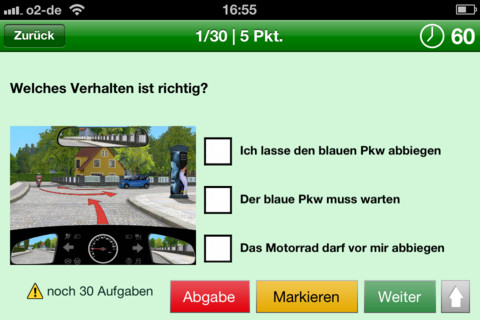
\includegraphics[width=0.7\textwidth]{../bilder/fahrschule_app.jpg} %70% der Textbreite
    	\caption{Beispielbild der Pocket Fahrschule Handy-Applikation}
    \end{figure}
\end{frame}

\begin{frame}
  \frametitle{Lernablauf - Intelligentes Tutorielles System}

  \begin{figure}[!htb]
  	\centering

  	\begin{tikzpicture}[->,>=stealth',
                      semithick]
  			\tikzstyle{comp2} = [fill=yellow, draw, rectangle, rounded corners, minimum height=0.8cm]
  			\tikzstyle{comp3} = [fill=black, text=white, draw, rectangle, rounded corners, minimum height=0.8cm]
  			\tikzstyle{comp1} = [draw, rectangle, rounded corners, minimum height=0.8cm]


        \node[comp1] (I) {Curriculum};
        \node[comp2] (A) [below=of I] {Erstelle Problem};
        \node[comp2] (B) [right=of A] {Präsentiere Problem};
        \node[comp2] (E) [right=of B] {Vergleiche Lösungen};
        \node[comp3] (C) [above=of E] {Student};
        \node[comp3] (D) [above left=of E] {Muster};
        \node[comp2] (F) [below=of E] {Analysiere Wissen};
        \node[comp2] (G) [left=of F] {Feedback};

  			\path (I) edge              (A)
  						(A) edge              (B)
  						(B) edge              (E)
  						(D) edge              (E)
  						(C) edge              (E)
  						(E) edge              (F)
  						(F) edge              (G)
  						(G) edge              (A);

  			\end{tikzpicture}
  \end{figure}

  \begin{columns}
    \begin{column}{0.5\textwidth}
       \begin{itemize}
         \item Feedback nach Wissensstand
         \item Lernproblem angepasst
       \end{itemize}
    \end{column}
    \begin{column}{0.5\textwidth}  %%<--- here
        \begin{itemize}
          \item flexibler Ablauf
          \item dauerhafte Re-Analyse
        \end{itemize}
    \end{column}
  \end{columns}
\end{frame}


\subsection{Architektur}
\subsection{Möglichkeiten zur Umsetzung von Adaption}


\section{Beispiel}
\subsection{LISP-Tutor}
\subsection{BRIDGE-Tutor}

\section{Fazit}

\end{document}
